\documentclass[12pt]{article}

\usepackage[a4paper,margin=2.54cm]{geometry}
\usepackage[T1]{fontenc}
\usepackage[utf8]{inputenc}
\usepackage{graphicx}
\usepackage{array}
\usepackage{booktabs}
\usepackage{hyperref}
\usepackage{float}
\usepackage{pgfplots}
\pgfplotsset{compat=1.18}

\linespread{1.5}
\setlength{\parindent}{0.5cm}
\setlength{\parskip}{0pt}

\title{SCML: Secure Context Mediation Layer\for Agentic AI and RAG Systems}
\author{Project Report}
\date{} 

\begin{document}

\begin{titlepage}
    \centering
    \vspace*{2cm}
    {\fontsize{20}{24}\selectfont \textbf{SCML: Secure Context Mediation Layer}}\\[0.6cm]
    {\fontsize{18}{22}\selectfont \textbf{for Agentic AI and RAG Systems}}\\[2cm]

    {\fontsize{14}{18}\selectfont Project Report}\\[3cm]

    {\fontsize{12}{16}\selectfont Department of Computer Science / AI Systems}\\[0.4cm]
    {\fontsize{12}{16}\selectfont Semester / Coursework Project}\\[0.4cm]
    {\fontsize{12}{16}\selectfont \today}\\[2cm]

    \vfill
\end{titlepage}

\tableofcontents
\clearpage

\section{Introduction}

Large language models (LLMs) are increasingly used in autonomous agents that interact with external tools, memory systems, and retrieval pipelines. These systems offer useful functionality, but they also introduce a significant security risk: untrusted or adversarial content can influence the agent's reasoning or its authorization decisions. In realistic deployments, an agent may read user messages, retrieved documents, memory records, or external web content and then decide whether to invoke a tool, write to memory, or emit a final answer. These flows are vulnerable to prompt injection, memory poisoning, and indirect data exfiltration attacks, especially when the model treats untrusted content as if it were trusted instructions.

This report presents SCML, the Secure Context Mediation Layer, as a middleware-based defense architecture that sits between an LLM agent and the components it reads from or acts upon. Rather than trying to make a model inherently robust to adversarial inputs, SCML treats security as a control-plane problem. It classifies data according to trust level, propagates taint values through the system, enforces least-agency policies before tool execution, quarantines suspicious memory writes, and redacts or blocks unsafe output. The project is implemented as a production-oriented Python system that exposes both client SDK and HTTP server interfaces, enabling deployment in agentic AI and RAG environments.

The system is grounded in the idea that external content can inform an agent without ever being allowed to authorize actions. This is the central invariant of the SCML design: untrusted data may affect what the system says or reasons about, but it must never directly enter the decision path for privileged operations such as tool calls or memory writes. The report describes the SCML architecture, the evaluation methodology, the benchmark datasets used, and the results obtained from the project’s security testing pipeline.

\section{Problem Statement \& Objectives}

The core problem addressed by SCML is that modern agentic systems often mix three kinds of data in the same operational context: trusted system instructions, user-supplied directives, and untrusted content from external sources. Once these are joined in a single prompt or shared memory store, a malicious payload may manipulate the model into disclosing secrets, triggering unauthorized commands, or altering long-term memory. This risk becomes more severe in retrieval-augmented systems, where documents retrieved from the web, internal knowledge stores, or third-party APIs may contain attacker-controlled instructions.

The problem is not limited to direct prompt injection. In multi-step agent workflows, memory poisoning is equally important. A malicious memory entry can influence future state, override policy assumptions, or create persistent malicious context. Likewise, model-generated output may leak sensitive content or embed adversarial instructions that later become trusted context. As a result, an effective security layer must protect not only the model input and output, but also the control flow that leads to tool invocation and memory mutation.

The main objectives of the project are therefore as follows:

\begin{itemize}
    \item To enforce trust-aware mediation between agent inputs, memory, and external tools.
    \item To distinguish between trusted instructions and untrusted data using taint propagation and label-based reasoning.
    \item To prevent prompt injection from influencing authorized actions by enforcing least-agency policies.
    \item To quarantine and review suspicious memory writes before they are persisted.
    \item To redact sensitive or dangerous output before it reaches a user or downstream system.
    \item To provide an auditable, tamper-evident decision trail using a chained audit log.
    \item To evaluate the system using benchmark-driven security testing across known injection and memory-poisoning datasets.
\end{itemize}

SCML is designed to tackle these problems using architecture-level mediation rather than model-only filtering. The design principle is to keep the agent useful while restricting the decisions that untrusted data may influence.

\section{Dataset Description}

The project does not rely on a single static dataset; instead, it uses benchmark-driven evaluation to measure security performance under real attack conditions. The dataset is composed of several security testbeds and benchmark suites that are bundled into the repository's evaluation harness. These include memory-poisoning evaluations, indirect-injection benchmarks, and agent benchmark suites used to measure both attack efficacy and utility retention.

\begin{table}[H]
\centering
\caption{Benchmark datasets and evaluation contexts used in the SCML project.}
\renewcommand{\arraystretch}{1.25}
\begin{tabular}{>{\raggedright\arraybackslash}p{3.3cm} >{\raggedright\arraybackslash}p{5.2cm} >{\raggedright\arraybackslash}p{5.4cm}}
\toprule
\textbf{Benchmark} & \textbf{Focus} & \textbf{Usage in SCML} \\
\midrule
Memory poisoning corpus & Malicious or deceptive memory writes designed to persist unsafe instructions across sessions & Measures storage-level ASR and harm-level impact under integrity checks \\
AgentDojo suite & Multi-tool agent tasks with adversarial attacks across domains & Compares defended vs. undefended system performance over attack scenarios and benign utility \\
InjecAgent benchmark & Third-party indirect-injection tasks (1054 cases) & Evaluates system-wide attack success rate, false-positive rate, and sensitivity to model and policy failures \\
Internal benchmark harness & Policy, tool-call, and output redaction scenarios & Validates adversarial inputs, memory integrity, and control-flow authorization \\
\bottomrule
\end{tabular}
\end{table}

The memory-poisoning benchmark is particularly relevant to the system's design because it specifically tests whether malicious state stored in memory can lead to unauthorized behavior later. In SCML, this is explicitly treated as a core integrity problem rather than merely a prompt-formatting issue. The AgentDojo suite provides a broader agentic test environment in which tools, external sources, and instruction-following are all present. InjecAgent offers a substantial third-party corpus of indirect-injection cases, which is useful for evaluating whether the defense remains effective on externally developed attack prompts rather than only on hand-crafted samples.

Taken together, these datasets capture the two dominant failure modes of agentic AI systems: (1) malicious content injected into prompts or retrieved documents and (2) adversarial influence stored in memory and later reintroduced into the control path. In a middleware-based solution, these datasets are essential because they test whether the agent is being protected at the right boundary.

\section{Exploratory Data Analysis}

The project includes an exploratory evaluation harness that aggregates attack-success measures, false positives, and utility trade-offs. The analysis shows that the dominant safety gain comes from least-agency enforcement and from limiting the influence of untrusted content on privileged operations. In the repository benchmark results, the system demonstrates meaningful reductions in attack success, but the measurements also show that no single mechanism eliminates all risk.

The first major outcome is that the memory integrity layer reduces attack success relative to an undefended baseline, but it does not fully eliminate the problem. The internal benchmark indicates that a substantial proportion of residual failures are concentrated in cases such as tool hijack and authority spoofing, which suggests that the current defense is most effective when policy enforcement and data classification are aligned with actual tool permissions. This result is important because it indicates that attack prevention in agentic systems depends on separating policy decisions from content interpretation.

The second major observation is that the benchmark results are highly sensitive to the distinction between storage contamination and harmful execution. A malicious memory record may be stored in a malicious state without being dangerous if the system never reads it in a privileged context. Conversely, a memory item can be harmless in storage yet become harmful when it reaches an authorization control point. SCML addresses this by enforcing a behavioural model in which untrusted or risky content may inform content generation but may not influence tool authorization or other side-effect operations.

Third, the results show a consistent trade-off between security and utility. In the AgentDojo evaluation, the defended system significantly reduces attack success, but some benign tasks that require fetching untrusted content or acting on external information are refused because they are semantically indistinguishable from attacks under the governance model. This is not a weakness in the system per se; rather, it is a consequence of least-agency enforcement. The system deliberately prefers denial over unauthorized action when the boundary between trusted and untrusted context is ambiguous.

These findings motivate the middleware approach. Security in agentic systems is not a single accuracy metric; it is a combination of attack resistance, false-positive discipline, auditability, and operational safety under ambiguity.

\section{Methodology}

The approach adopted in SCML is a layered security pipeline built around trust mediation and least-privilege design. The methodology is operationalized through the following stages:

\begin{enumerate}
    \item \textbf{Trust classification and taint propagation.} All incoming data is assigned a trust label such as trusted, untrusted, or risky external. The label is propagated to derived values so that downstream reasoning preserves the highest-risk classification.
    \item \textbf{Ingress control and routing.} The incoming prompt, retrieved document, or memory record is routed through the mediator before it reaches the agent or policy engine. This prevents untrusted payloads from being mixed directly into privileged control logic.
    \item \textbf{Injection scanning.} The system applies heuristic and classifier-based scanning to detect prompt injection patterns and malicious instructions. The scanner identifies suspicious content before tool authorization is considered.
    \item \textbf{Tool-policy enforcement.} Tool calls are checked against declarative allow-lists, high-impact safeguards, and rate limits. This is the main control point for preventing indirect prompt injection from causing side effects.
    \item \textbf{Memory integrity validation.} Candidate writes are quarantined and assessed before they are persisted. If a memory item is deceptive or malicious, it is refused or isolated for review.
    \item \textbf{Output mediation and redaction.} Before response generation or external transmission, the system checks for secrets, sensitive information, or injection-like content that should not be exposed.
    \item \textbf{Audit logging and forensic verification.} Every decision is recorded in a hash-chained audit log to support later forensic review and tamper detection.
\end{enumerate}

This methodology is more robust than simple prompt filtering because it places enforcement at system boundaries: the control plane is protected even when the content plane remains noisy or adversarial. The architecture therefore aligns with established security principles of least privilege, fail-closed behavior, and explicit trust boundaries.

\section{Solution Implementation / Model Development}

The SCML implementation is organized as a modular Python project with a thin client SDK and a server-side mediator. The root package exposes a public client API while keeping the internal service stack separate. The project includes the core modules responsible for ingress handling, trust routing, injection scanning, tool-policy management, memory integrity checks, output redaction, audit logging, and policy storage.

The main implementation structure is as follows:

\begin{itemize}
    \item \textbf{trust\_mediator/client.py} provides the SCML client library and normalizes the HTTP responses from multiple mediator endpoints. This ensures that callers do not need to branch on different response shapes depending on whether the API returns a decision, a verdict, or a blocked flag.
    \item \textbf{trust\_mediator/core/pipeline.py} orchestrates the full mediation pipeline, combining trust labeling, scanning, policy checks, memory integrity checks, and audit decisions.
    \item \textbf{trust\_mediator/modules/} implements the eight functional components specified by the project architecture, including the injection scanner, tool policy engine, and memory integrity layer.
    \item \textbf{trust\_mediator/api/} exposes the mediator through FastAPI endpoints and optional gRPC support.
    \item \textbf{benchmarks/} contains the security evaluation harness and benchmark suites for measuring attack success, false positives, and latency.
\end{itemize}

The system uses declarative policies to express allowed tools, agent-specific authorizations, and review workflows. This constrains the agent's authority and prevents cross-agent privilege leakage. In production, the mediation component supports deployment via Docker Compose, FastAPI, and optional gRPC transport. The project also includes a TypeScript client and optional LangChain integration, making it usable across both Python and JavaScript ecosystems.

The model-development aspect of the project is not a single monolithic model; instead, it is a policy-and-classification architecture. The injection scanner supports heuristic checks and pluggable ML classifiers, while the tool policy layer is rule-based and declarative. This separation is a deliberate design decision: static policy enforcement is stronger and more predictable than relying solely on a classification model for authorization.

\section{Results \& Discussion}

The results in the repository show that SCML provides meaningful protection against indirect prompt injection and memory-poisoning attacks, while also highlighting the limits of any single-layer defense. Selected benchmark results are summarized below and presented in figures that emphasize both the reduction in attack success and the trade-off in operational utility.

\begin{figure}[H]
\centering
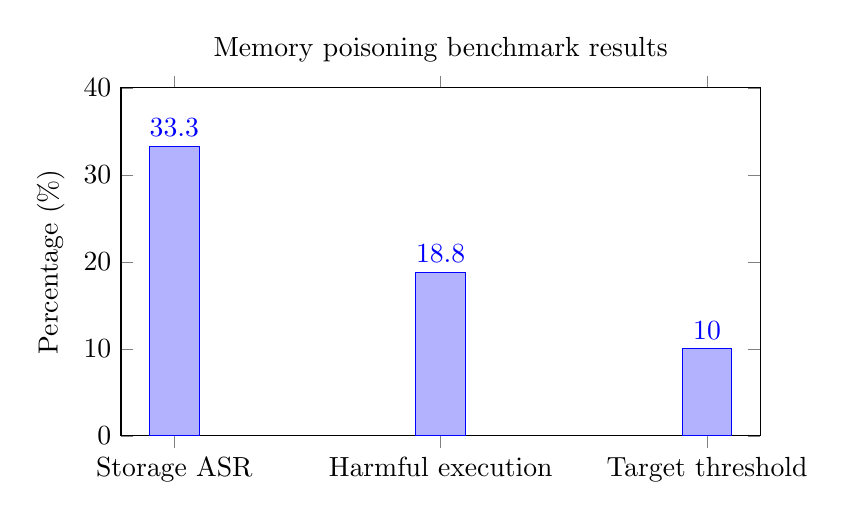
\begin{tikzpicture}
\begin{axis}[
    width=0.8\linewidth,
    height=6cm,
    ybar,
    symbolic x coords={Storage ASR,Harmful execution,Target threshold},
    xtick=data,
    ylabel={Percentage (\%)},
    ymin=0,
    ymax=40,
    nodes near coords,
    bar width=18pt,
    title={Memory poisoning benchmark results}
]
\addplot coordinates {(Storage ASR,33.3) (Harmful execution,18.8) (Target threshold,10.0)};
\end{axis}
\end{tikzpicture}
\caption{Memory poisoning benchmark results showing attack success rate and harmful execution relative to the threshold target.}
\end{figure}

\begin{figure}[H]
\centering
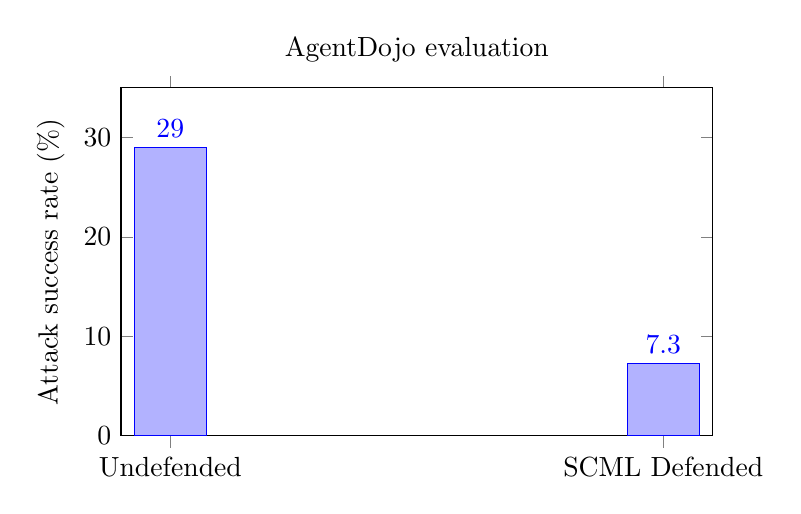
\begin{tikzpicture}
\begin{axis}[
    width=0.75\linewidth,
    height=6cm,
    ybar,
    symbolic x coords={Undefended,SCML Defended},
    xtick=data,
    ylabel={Attack success rate (\%)},
    ymin=0,
    ymax=35,
    nodes near coords,
    bar width=26pt,
    title={AgentDojo evaluation}
]
\addplot coordinates {(Undefended,29.0) (SCML Defended,7.3)};
\end{axis}
\end{tikzpicture}
\caption{Comparison of attack success rate between the undefended baseline and the SCML-mediated defense in the AgentDojo benchmark.}
\end{figure}

\begin{table}[H]
\centering
\caption{Selected benchmark outcomes reported in the SCML project.}
\renewcommand{\arraystretch}{1.3}
\begin{tabular}{>{\raggedright\arraybackslash}p{3.5cm} >{\raggedright\arraybackslash}p{3.5cm} >{\raggedright\arraybackslash}p{5.8cm}}
\toprule
\textbf{Evaluation} & \textbf{Reported result} & \textbf{Interpretation} \\
\midrule
Memory poisoning (storage) & 33.3\% ASR vs. $<$10\% target & Shows improvement but does not yet reach production acceptance for the full memory-integrity objective \\
Memory poisoning (harm) & 18.8\% harmful score across evaluated cases & Indicates that the system blocks most harmful action paths, while some attacks remain under the current detector coverage \\
AgentDojo & 29.0\% $\rightarrow$ 7.3\% attack success, with utility retained at 81\% defended vs. baseline range & Demonstrates strong reduction in attack success with a measurable utility trade-off \\
InjecAgent & 1054 indirect-injection cases; all five KPI targets pass under the project evaluation & Shows that the policy layer is the dominant defense, while scanner detection alone is not sufficient for attack coverage \\
\bottomrule
\end{tabular}
\end{table}

These findings suggest several important conclusions. First, the strongest defense is not the model itself but the authorization and trust boundary enforced by SCML. The project explicitly treats tool calls and memory writes as privileged operations that must remain independent from untrusted data. This is consistent with the architectural rule that untrusted content may inform the content of a response but must not authorize side effects.

Second, the results reveal that detection by itself is insufficient. In the InjecAgent benchmark, the injection scanner does not materially detect the attacks, yet overall harmful execution remains low because the tool-policy layer enforces least agency. This demonstrates that the largest security gain comes from restricting what the model is allowed to do, not merely from trying to identify malicious instructions.

Third, the benchmark results establish that utility and security are not identical objectives. A stricter policy reduces attack success but may also reject some benign tasks that require external data access. This is a deliberate consequence of fail-closed mediation and is consistent with secure deployment design in high-risk agent workflows.

The discussion should therefore not frame SCML as a complete removal of risk. Instead, SCML is best understood as a practical control layer that implements the principle of least agency in a way that can be integrated into existing agentic and RAG systems. It reduces adversarial influence at the system boundary, creates explicit trust labels, and preserves an auditable record of all decisions.

\section{Conclusion}

This project presents SCML as a secure middleware architecture for agentic AI and retrieval-based systems. The main contribution is not a single classifier or a one-off prompt-defense technique, but a system-level approach that separates content generation from privileged control decisions. By classifying inputs, propagating trust labels, enforcing policy at tool-call boundaries, validating memory writes, and redacting unsafe output, SCML creates a robust security layer for autonomous systems.

The report also shows that the design is informed by real benchmark evaluation. The project's benchmark suite includes memory-poisoning and indirect-injection tests that reveal both the strengths and the current limitations of the system. The strongest observed protection comes from tool-policy enforcement and least-agency control, while the remaining attack surface is concentrated in cases where an attacker influences memory or payload interpretation across several steps of the workflow.

SCML is therefore best viewed as a practical and deployable mediation layer rather than a purely academic defense. It balances security, auditability, and usability, and it directly addresses the operational reality of modern AI agents: they must read untrusted content, act on external information, and still remain safe under adversarial conditions. The project demonstrates that meaningful protection can be achieved by making the trust boundary explicit and enforcing it consistently across the whole system lifecycle.

\section{References}

\begin{thebibliography}{9}
\bibitem{prdv1} TrustMediator Project. \emph{TrustMediator PRD v1.0}. Project specification, 2026.
\bibitem{addendum} TrustMediator Project. \emph{PRD v1.1 Addendum}. Security benchmark and acceptance criteria update, 2026.
\bibitem{readme} TrustMediator Project. \emph{README and Project Architecture Documentation}. Repository documentation, 2026.
\bibitem{bench} TrustMediator Project. \emph{Benchmark Harness and Evaluation Results}. Benchmarks directory and result reports, 2026.
\bibitem{greshake2023} Greshake, K., et al. \emph{More than you’ve asked for: A Comprehensive Analysis of Prompt Injection Threats Against GPT-based Systems}. 2023.
\bibitem{liu2024} Liu, Y., et al. \emph{Prompt Injection Attack against LLM-Integrated Applications}. 2024.
\bibitem{zou2024} Zou, A., et al. \emph{PoisonedRAG: How Retrieval-Augmented Generation Poisoning Attacks Target LLMs}. 2024.
\bibitem{debenedetti2024} Debenedetti, E., et al. \emph{AgentDojo: A Dynamic Environment to Evaluate Tool-Use in LLM Agents}. 2024.
\bibitem{injecagent} Mosaic Lab / benchmark team. \emph{InjecAgent: Indirect Injection Evaluation Corpus}. 2024.
\bibitem{owasp2025} OWASP Foundation. \emph{OWASP Top 10 for Large Language Model Applications}. 2025.
\end{thebibliography}

\end{document}
